%%%%%%%%%%%%%%%%%%%%%%%%%%%%%%%%%%%%%%%%%%%%%%%%%
%%%
%%% SIGBOVIK 2020 TRIPLE BLIND REVIEW TEMPLATE
%%%
%%% Instructions:
%%%
%%% 1. Edit the author, rating, and confidence
%%%    fields.
%%% 2. Enter your review after the \maketitle
%%%    command
%%%
%%%%%%%%%%%%%%%%%%%%%%%%%%%%%%%%%%%%%%%%%%%%%%%%%
\documentclass[12pt]{sigbovik-review}
\usepackage{graphicx}
%%%% Edit the following three lines.
%% To ensure the integrity of the triple-blind review
%% process, the contents of the \author field should not
%% reveal your identity.
\author{Definitely not the SIGBOVIK webmaster}
\rating{3rd grade reading comprehension}
\confidence{Confident that some cool people said to email reviews to \\the sigbovik-reviews mailing list and \emph{not} to easychair}

%%%% The Proceedings Chair will fill in the following
%%%% two fields.
\papernum{NN}
\papertitle{UNKNOWN PAPER TITLE}

\begin{document}

\maketitle

%%% Replace the following text with your review.
\begin{figure}[!h]
\centering
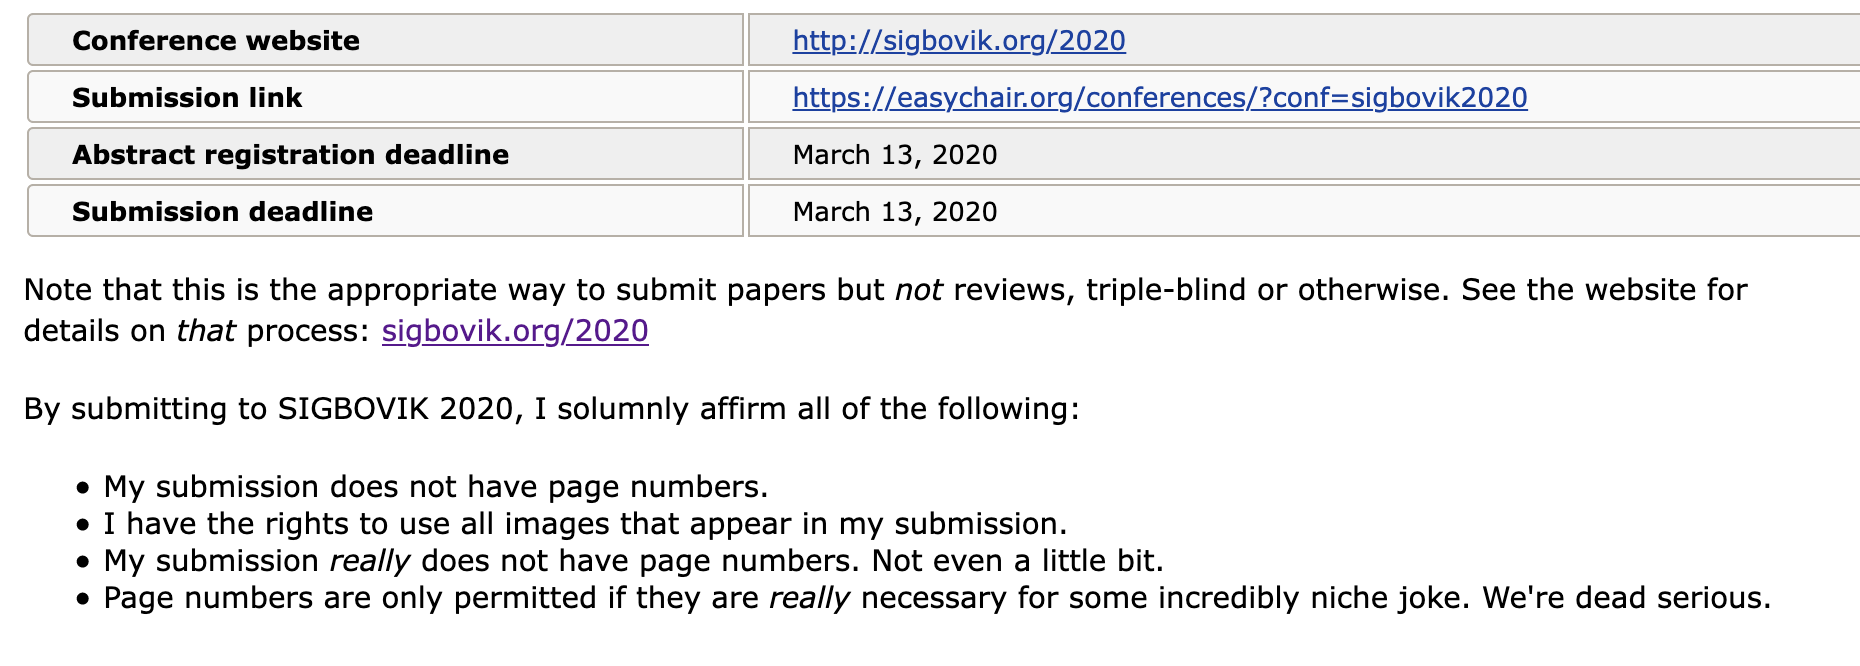
\includegraphics[width=.9\textwidth]{easychair}
\caption{The easychair \emph{paper} submission site}
\end{figure}

\begin{figure}[!h]
\centering
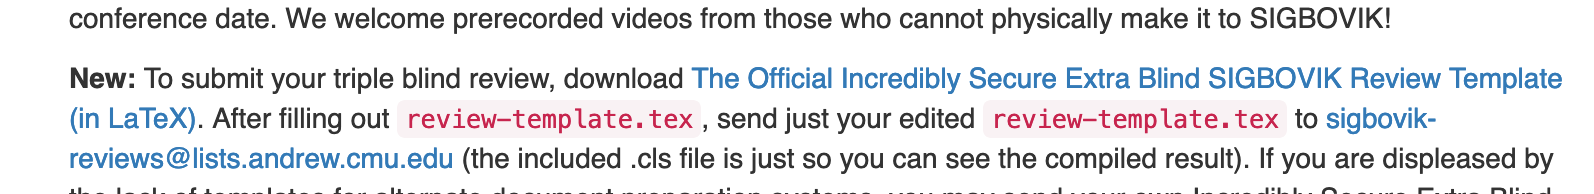
\includegraphics[width=.9\textwidth]{website}
\caption{The SIGBOVIK 2020 website instructions for submitting reviews}
\end{figure}

\end{document}